
\begin{frame}
\frametitle{Curse of dimensionality}
\begin{center}
{\Huge Large $p$, small $n$.\par}
\end{center}
\end{frame}

\begin{frame}
\frametitle{Nearest-neighbour classification}
\begin{columns}[c]
\column{0.7\textwidth}
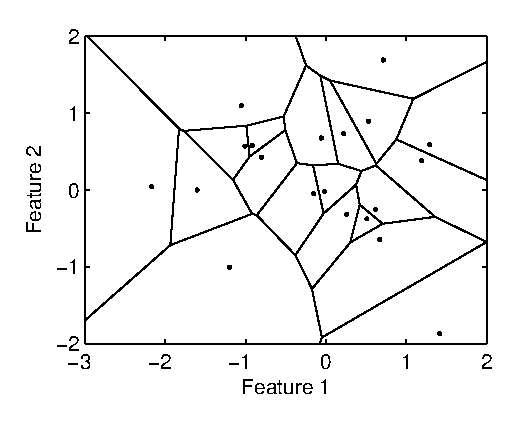
\includegraphics[width=\textwidth]{voronoi}
\column{0.3\textwidth}
\begin{itemize}
\item Not nice smooth separations.
\item Lots of sharp corners.
\item May be improved with \emph{K-nearest neighbours}.
\end{itemize}
\end{columns}
\end{frame}

\begin{frame}
\frametitle{Rule-based approaches}
\begin{columns}[c]
\column{0.7\textwidth}
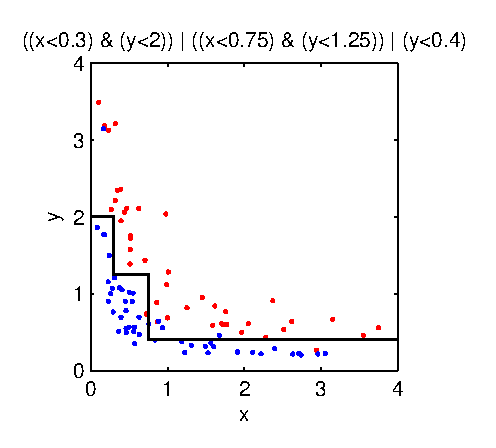
\includegraphics[width=\textwidth]{rule_based}
\column{0.3\textwidth}
\begin{itemize}
\item Not nice smooth separations.
\item Lots of sharp corners.
\end{itemize}
\end{columns}
\end{frame}


\begin{frame}
\frametitle{Corners matter in high-dimensions}
\begin{columns}[c]
\column{0.4\textwidth}
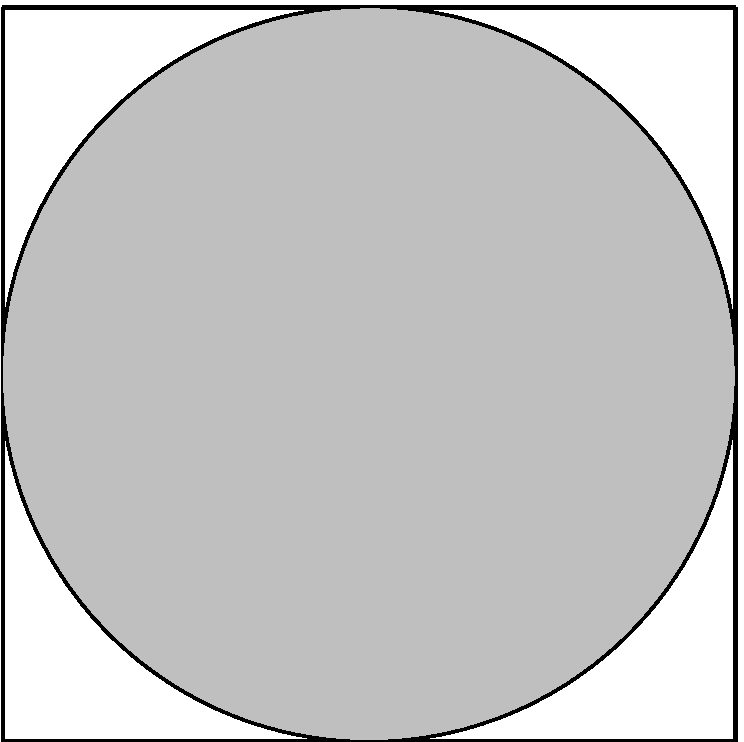
\includegraphics[width=\textwidth]{circle}
\column{0.6\textwidth}
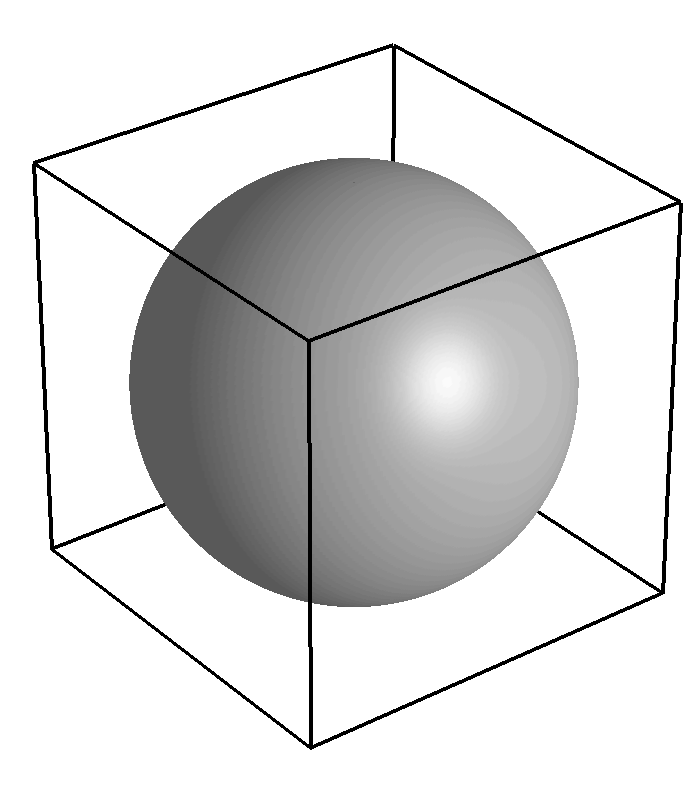
\includegraphics[width=\textwidth]{sphere}
\end{columns}
\end{frame}

\begin{frame}
\frametitle{Corners matter in high-dimensions}
\begin{columns}[c]
\column{0.2\textwidth}
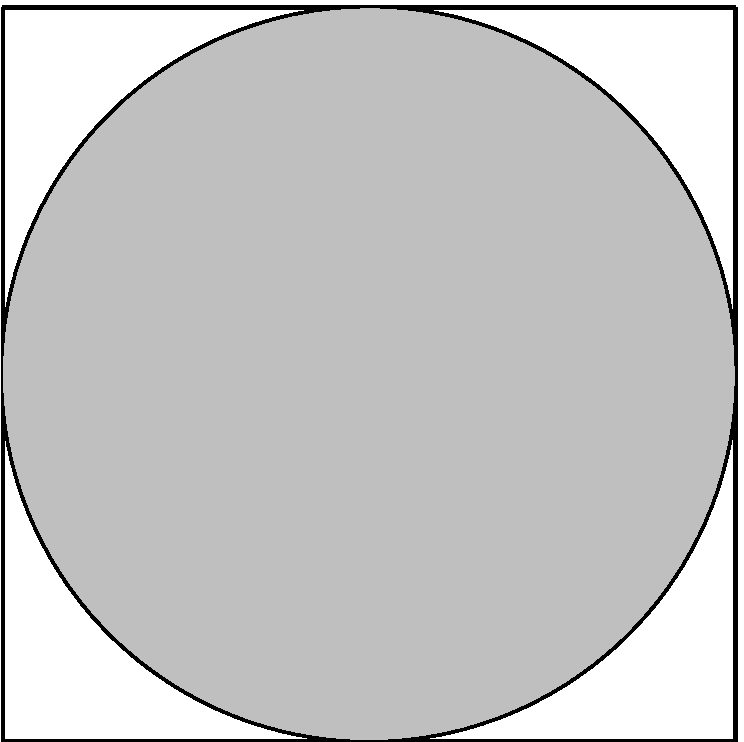
\includegraphics[width=.8\textwidth]{circle}

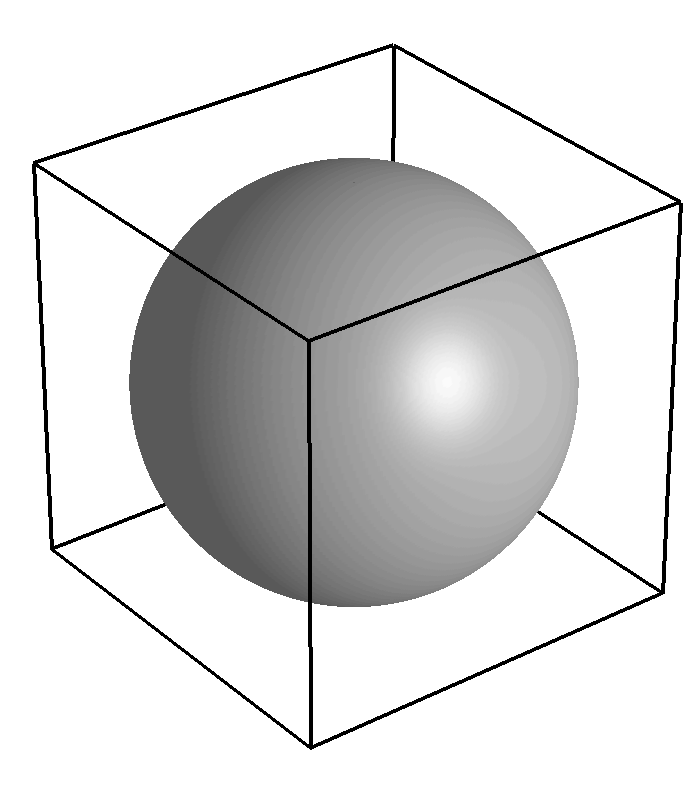
\includegraphics[width=\textwidth]{sphere}
\column{0.8\textwidth}
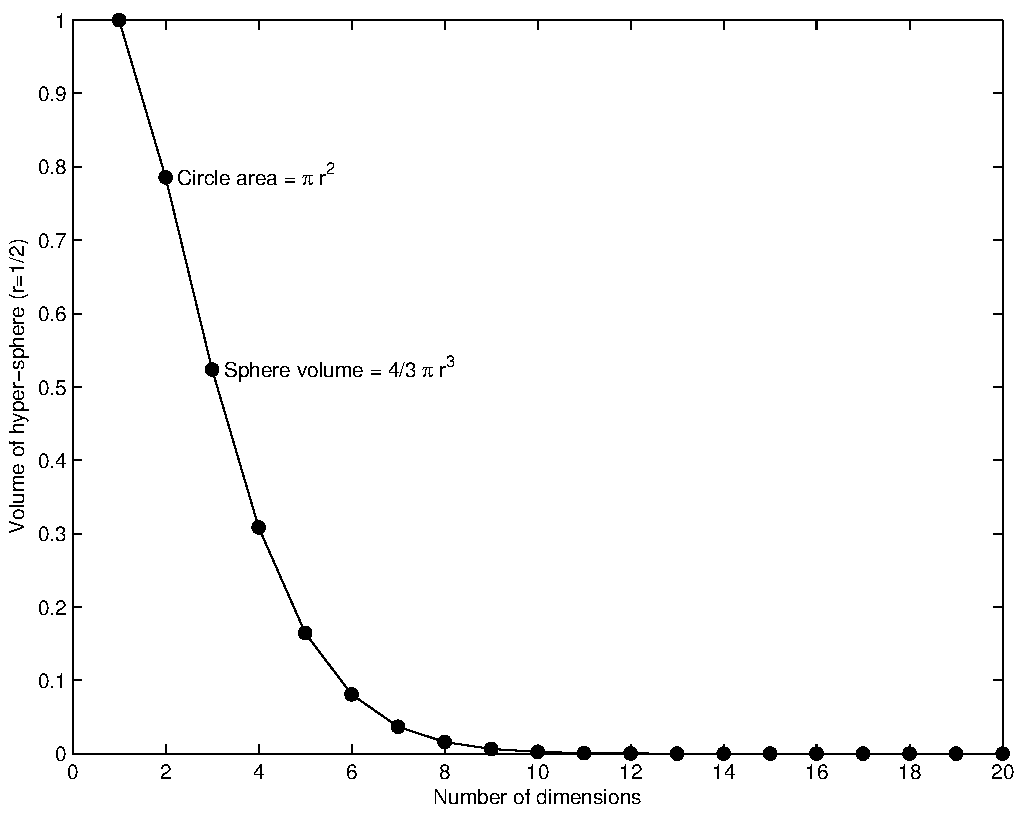
\includegraphics[width=\textwidth]{corners}
\end{columns}
\end{frame}


\begin{frame}
\frametitle{Dimensionality $\ne$ number of voxels}
\begin{itemize}
\item Lots of effort on data-driven feature selection methods.
\begin{itemize}
\item Involves estimating weighting matrix such that\\
      ${\bf W} = diag({\bf w}), w_i \in \{0,1\}$.
\item Lots of parameters needed to achieve this.
\end{itemize}
\item Many papers claim excellent results.
\item Little evidence to suggest that most voxel-based feature selection methods help.
\begin{itemize}
\item Little or no increase in predictive accuracy.
\item Commonly perceived as being more ``interpretable''.
\end{itemize}
%\item Prior knowledge derived from independent data is the most reliable way to improve accuracy.
%\begin{itemize}
%\item e.g. search the literature for clues about which regions to weight more heavily.
%\end{itemize}
\end{itemize}
\end{frame}

\begin{frame}
%\frametitle{Credentials}
\begin{center}
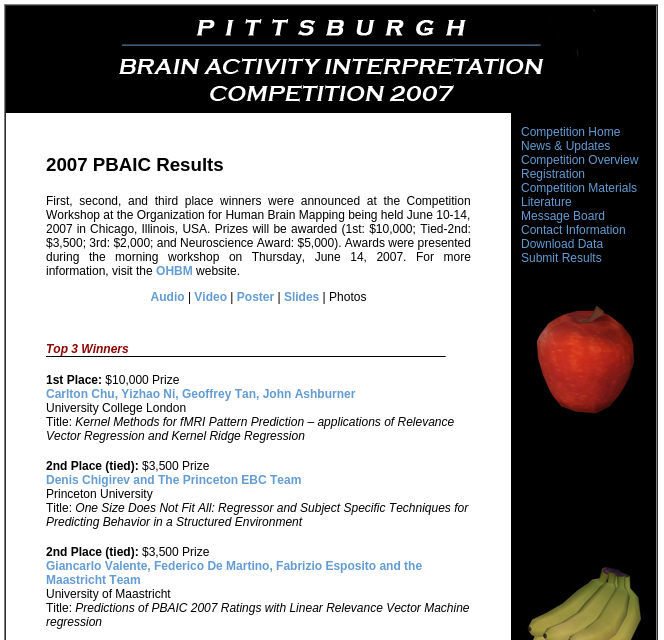
\includegraphics[height=0.7\textwidth]{pbaic2007}
\end{center}
\end{frame}

\begin{frame}
%\frametitle{Credentials}
\begin{center}
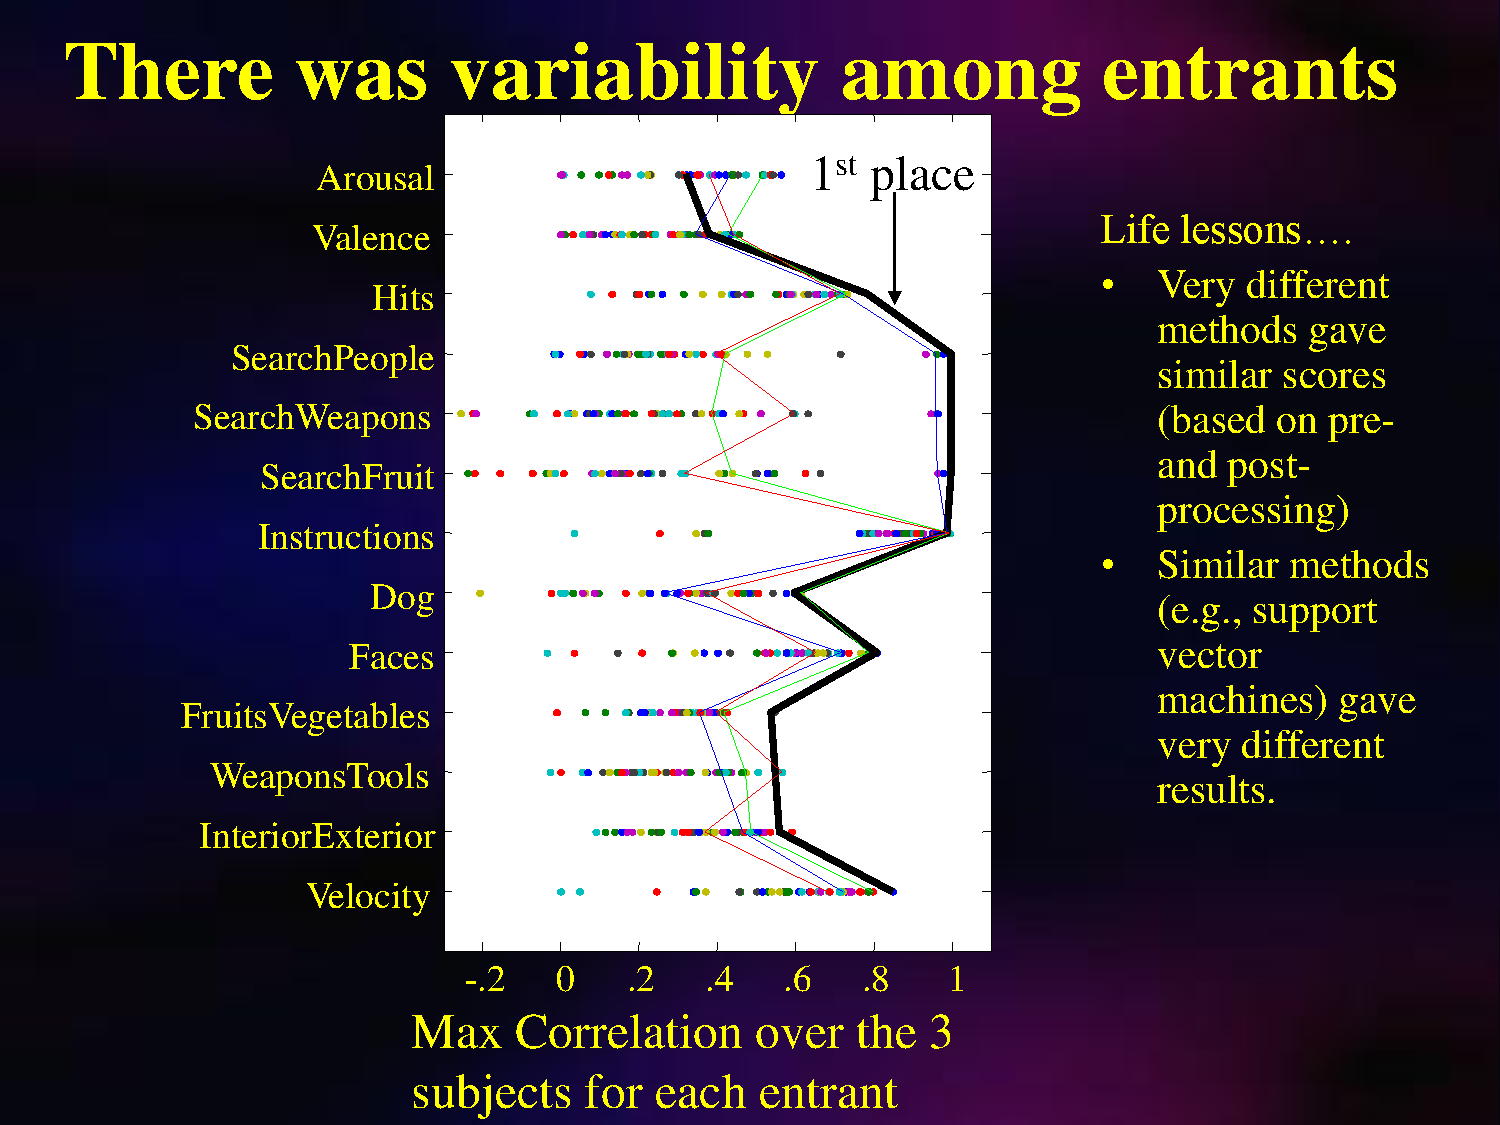
\includegraphics[height=0.7\textwidth]{pbaic2007_2}
\end{center}
\end{frame}


%\begin{frame}
%\frametitle{Data-driven feature selection}
%\begin{itemize}
%\item Lots of effort on data-driven feature selection methods.
%\item Many papers claim excellent results.
%\item Not much evidence that it really improves accuracy.
%\end{itemize}
%\end{frame}

\begin{frame}
\frametitle{Data-driven feature selection}
%The main objectives of the feature selection step are to keep only informative features and to reduce the dimensionality of the feature space.
\begin{quote}
``In our evaluation, two methods included a feature selection step: Voxel-STAND and Voxel-COMPARE.
Overall, these methods did not perform substantially better than simpler ones... ...
%In particular, their results might be more sensitive to the training set.
%Indeed, feature selection can be regarded as a learning step.
%In such a case, the feature selection step increases the class of all possible classification functions, which could lead to overfitting the data.
A more robust way to decrease the dimensionality of the features way would be to use more prior knowledge of the disease.''

%Besides features selection can be time consuming as it adds new hyperparameters and thus makes the grid search less tractable.
%Compared to Voxel-Direct and Voxel-Atlas, Voxel-STAND and Voxel-COMPARE are time consuming (up to weeks), mostly because of the number of hyperparameters to be tuned.

%Nevertheless, feature selection proved useful in two specific cases.
%First, these methods proved less sensitive when increasing the dimensionality of the feature space by adding WM and CSF maps.
%They also tended to be more accurate for the MCIc vs MCInc experiment, where only a few brain regions are informative.
\end{quote}

\begin{center}
\begin{tiny}
Cuingnet et al. ``Automatic classification of patients with Alzheimer's disease from structural MRI: A comparison of ten methods using the ADNI database''.  NeuroImage 56(2):766--781 (2011).\par
\end{tiny}
\end{center}
\end{frame}

\begin{frame}
\frametitle{Data-driven feature selection}
\begin{center}
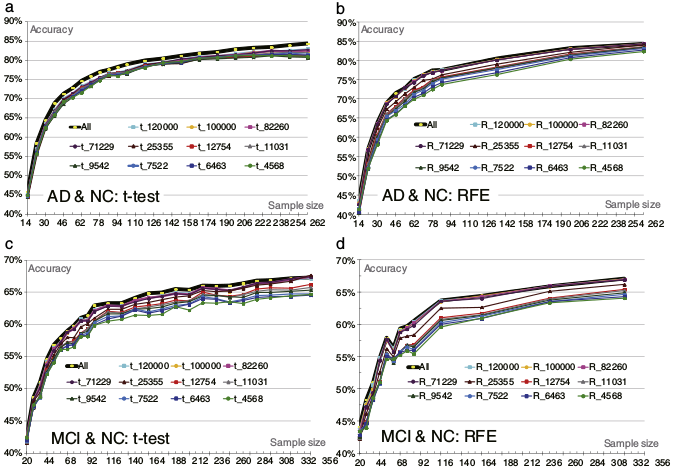
\includegraphics[height=0.55\textwidth]{data_driven_feature_selection.png}\par
\begin{tiny}
Chu et al. ``Does feature selection improve classification accuracy? Impact of sample size and feature selection on classification using anatomical magnetic resonance images''.  NeuroImage 60:59--70 (2012).\par
\end{tiny}
\end{center}
\end{frame}

\begin{frame}
\frametitle{One mode of geometric variability}
\begin{columns}[c]
\column{0.5\textwidth}
Simulated images\par
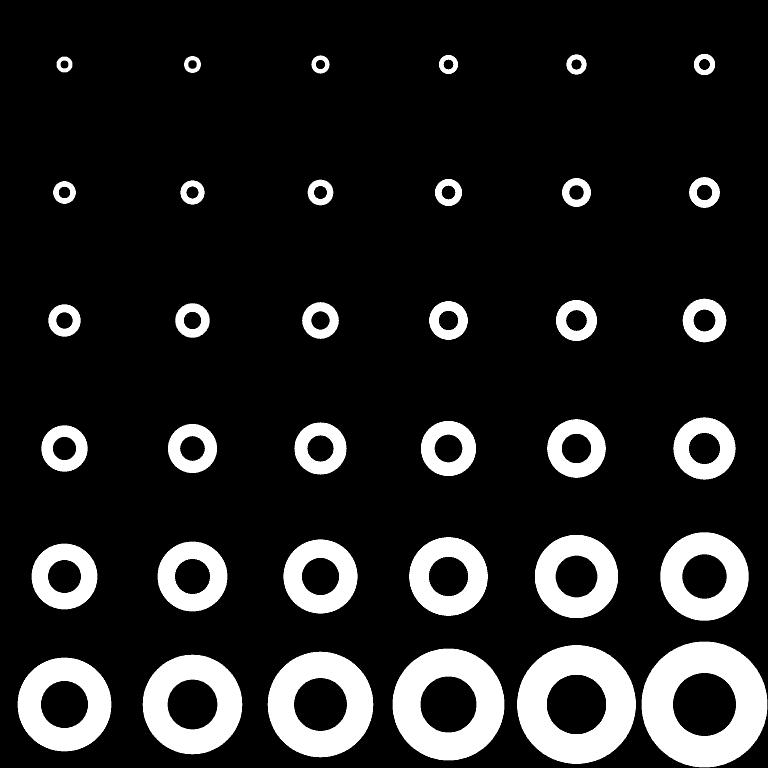
\includegraphics[height=0.9\textwidth]{circles}
\column{0.5\textwidth}
Principal components\par
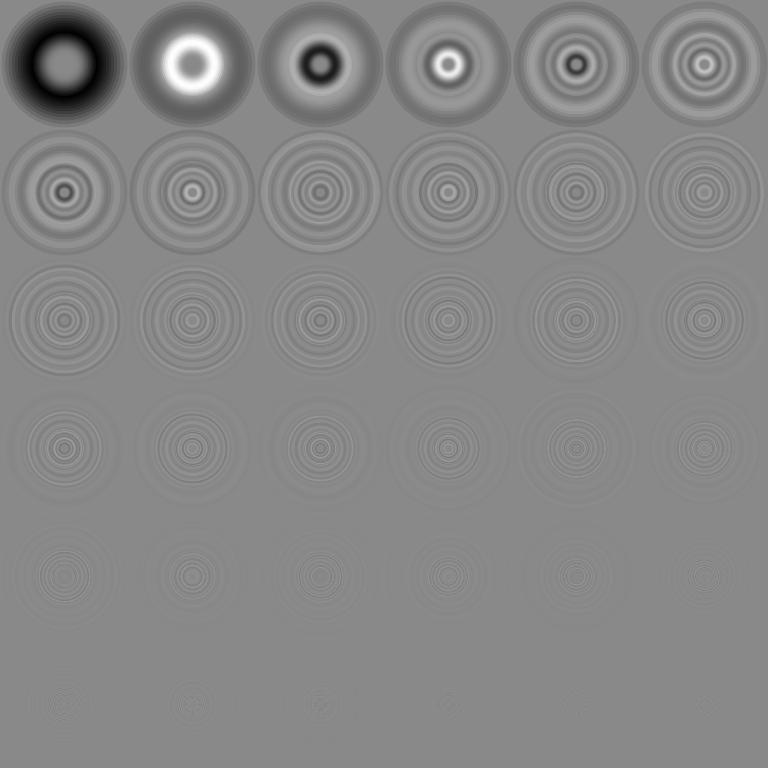
\includegraphics[height=0.9\textwidth]{circles_pca}
\end{columns}
A suitable model would reduce these data to a single dimension.
\end{frame}


\begin{frame}
\frametitle{Two modes of geometric variability}
\begin{columns}[c]
\column{0.5\textwidth}
Simulated images\par
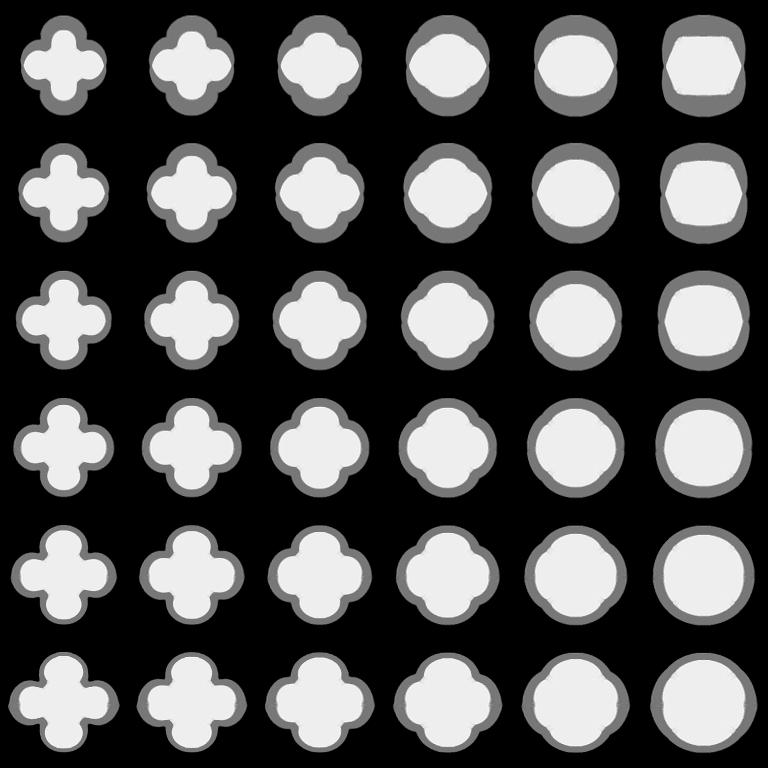
\includegraphics[height=0.9\textwidth]{things}
\column{0.5\textwidth}
Principal components\par
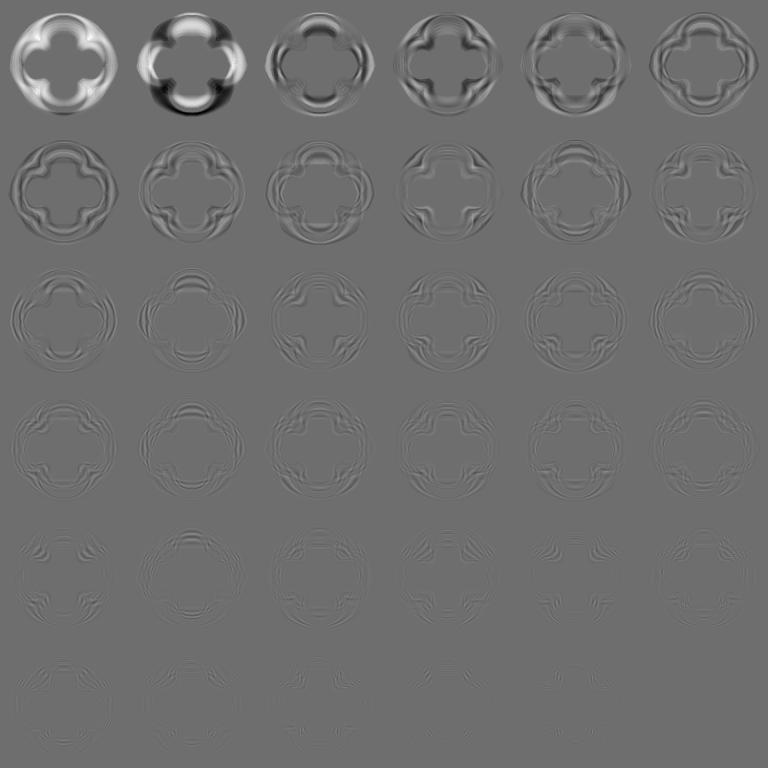
\includegraphics[height=0.9\textwidth]{things_pca}
\end{columns}
A suitable model would reduce these data to two dimensions.
\end{frame}

